\documentclass[newPxFont]{beamer}\usepackage[]{graphicx}\usepackage[]{color}
%% maxwidth is the original width if it is less than linewidth
%% otherwise use linewidth (to make sure the graphics do not exceed the margin)
\makeatletter
\def\maxwidth{ %
  \ifdim\Gin@nat@width>\linewidth
    \linewidth
  \else
    \Gin@nat@width
  \fi
}
\makeatother

\definecolor{fgcolor}{rgb}{0.345, 0.345, 0.345}
\newcommand{\hlnum}[1]{\textcolor[rgb]{0.686,0.059,0.569}{#1}}%
\newcommand{\hlstr}[1]{\textcolor[rgb]{0.192,0.494,0.8}{#1}}%
\newcommand{\hlcom}[1]{\textcolor[rgb]{0.678,0.584,0.686}{\textit{#1}}}%
\newcommand{\hlopt}[1]{\textcolor[rgb]{0,0,0}{#1}}%
\newcommand{\hlstd}[1]{\textcolor[rgb]{0.345,0.345,0.345}{#1}}%
\newcommand{\hlkwa}[1]{\textcolor[rgb]{0.161,0.373,0.58}{\textbf{#1}}}%
\newcommand{\hlkwb}[1]{\textcolor[rgb]{0.69,0.353,0.396}{#1}}%
\newcommand{\hlkwc}[1]{\textcolor[rgb]{0.333,0.667,0.333}{#1}}%
\newcommand{\hlkwd}[1]{\textcolor[rgb]{0.737,0.353,0.396}{\textbf{#1}}}%

\usepackage{framed}
\makeatletter
\newenvironment{kframe}{%
 \def\at@end@of@kframe{}%
 \ifinner\ifhmode%
  \def\at@end@of@kframe{\end{minipage}}%
  \begin{minipage}{\columnwidth}%
 \fi\fi%
 \def\FrameCommand##1{\hskip\@totalleftmargin \hskip-\fboxsep
 \colorbox{shadecolor}{##1}\hskip-\fboxsep
     % There is no \\@totalrightmargin, so:
     \hskip-\linewidth \hskip-\@totalleftmargin \hskip\columnwidth}%
 \MakeFramed {\advance\hsize-\width
   \@totalleftmargin\z@ \linewidth\hsize
   \@setminipage}}%
 {\par\unskip\endMakeFramed%
 \at@end@of@kframe}
\makeatother

\definecolor{shadecolor}{rgb}{.97, .97, .97}
\definecolor{messagecolor}{rgb}{0, 0, 0}
\definecolor{warningcolor}{rgb}{1, 0, 1}
\definecolor{errorcolor}{rgb}{1, 0, 0}
\newenvironment{knitrout}{}{} % an empty environment to be redefined in TeX

\usepackage{alltt}
\usetheme{sthlm}
%\usecolortheme{sthlmv42}


%-=-=-=-=-=-=-=-=-=-=-=-=-=-=-=-=-=-=-=-=-=-=-=-=
%        LOADING PACKAGES
%-=-=-=-=-=-=-=-=-=-=-=-=-=-=-=-=-=-=-=-=-=-=-=-=
\usepackage[utf8]{inputenc}
% \usepackage{mathpazo}
\usepackage{chronology}
\usepackage[natbib=true, backend=bibtex, style=numeric, citestyle=numeric]{biblatex}
\usepackage{apalike}
\usepackage{fix-cm}
\usepackage{pgf, tikz}
\usetikzlibrary{positioning, shapes, fit, chains}

%% Some Customizations and loadings
\addbibresource{references.bib}
\renewcommand\bibfont{\scriptsize}
% If you have more than one page of references, you want to tell beamer
% to put the continuation section label from the second slide onwards
\setbeamertemplate{frametitle continuation}[from second]
% Now get rid of all the colours
\setbeamercolor*{bibliography entry title}{fg=black}
\setbeamercolor*{bibliography entry author}{fg=black}
\setbeamercolor*{bibliography entry location}{fg=black}
\setbeamercolor*{bibliography entry note}{fg=black}
% and kill the abominable icon
\setbeamertemplate{bibliography item}{\insertbiblabel}
\setbeamertemplate{caption}[numbered, justification=centering]
\setbeamerfont{caption}{size=\scriptsize}

\renewcommand{\event}[3][e]{%
  \pgfmathsetlength\xstop{(#2-\theyearstart)*\unit}%
  \ifx #1e%
    \draw[fill=black,draw=none,opacity=0.5]%
      (\xstop, 0) circle (.2\unit)%
      node[opacity=1,rotate=45,right=.2\unit] {#3};%
  \else%
    \pgfmathsetlength\xstart{(#1-\theyearstart)*\unit}%
    \draw[fill=black,draw=none,opacity=0.5,rounded corners=.1\unit]%
      (\xstart,-.1\unit) rectangle%
      node[opacity=1,rotate=45,right=.2\unit] {#3} (\xstop,.1\unit);%
  \fi}%


\title{Models Can Lie}
\subtitle{An Illustration from Heart Rate Variablity Data}
%\date{\small{\jobname}}
\date{\today}
\author{Raju Rimal and Veronika Lindberg}
\institute{Norwegian University of Science and Technology \\
\large{Norwegian University of Life Sciences}}

\hypersetup{
pdfauthor = {Raju Rimal},
pdftitle = {Models Can Lie},
pdfsubject = {Statistics},
pdfkeywords = {},
pdfmoddate= {D:\pdfdate},
pdfcreator = {}
}
\IfFileExists{upquote.sty}{\usepackage{upquote}}{}
\begin{document}

%-=-=-=-=-=-=-=-=-=-=-=-=-=-=-=-=-=-=-=-=-=-=-=-=
%
%	TITLE PAGE
%
%-=-=-=-=-=-=-=-=-=-=-=-=-=-=-=-=-=-=-=-=-=-=-=-=

\maketitle

%-=-=-=-=-=-=-=-=-=-=-=-=-=-=-=-=-=-=-=-=-=-=-=-=
%
%	Initial Stuffs
%
%-=-=-=-=-=-=-=-=-=-=-=-=-=-=-=-=-=-=-=-=-=-=-=-=





%-=-=-=-=-=-=-=-=-=-=-=-=-=-=-=-=-=-=-=-=-=-=-=-=
%
%	TABLE OF CONTENTS: OVERVIEW
%
%-=-=-=-=-=-=-=-=-=-=-=-=-=-=-=-=-=-=-=-=-=-=-=-=
\begin{frame}{Overview}
\tableofcontents
\end{frame}

\section{Background}
%-=-=-=-=-=-=-=-=-=-=-=-=-=-=-=-=-=-=-=-=-=-=-=-=
%	FRAME: Some Background
%-=-=-=-=-=-=-=-=-=-=-=-=-=-=-=-=-=-=-=-=-=-=-=-=
\begin{frame}[c, fragile]{Some Background}
\begin{enumerate}[<+->]
  \item PCR, PLS and Canonically Powered PLS (CPPLS) is used in the analysis
  \item CPPLS integrate CCA with PLS to select relevant variables for response
  \item Cross-validation is performed over the observations on each a) frequency window b) series c) person-event combination
  \item Three variation of dataset is used
  \begin{itemize}
   \item Transpose of each frequency windows stacked together
   \item The average frequencies over time for each Series
   \item The average frequencies over time for each person-event combination
  \end{itemize}
  \item LDA model is used for discriminant analysis using the scores obtained form each of the latent variable model with cross-validation implemented
\end{enumerate}
\end{frame}

\section{How data looks like}
%-=-=-=-=-=-=-=-=-=-=-=-=-=-=-=-=-=-=-=-=-=-=-=-=
%	FRAME: How data looks like
%-=-=-=-=-=-=-=-=-=-=-=-=-=-=-=-=-=-=-=-=-=-=-=-=



\begin{frame}[t]{How data looks like}
\begin{columns}[t]
\column{0.7\textwidth}
\begin{knitrout}
\definecolor{shadecolor}{rgb}{0.969, 0.969, 0.969}\color{fgcolor}
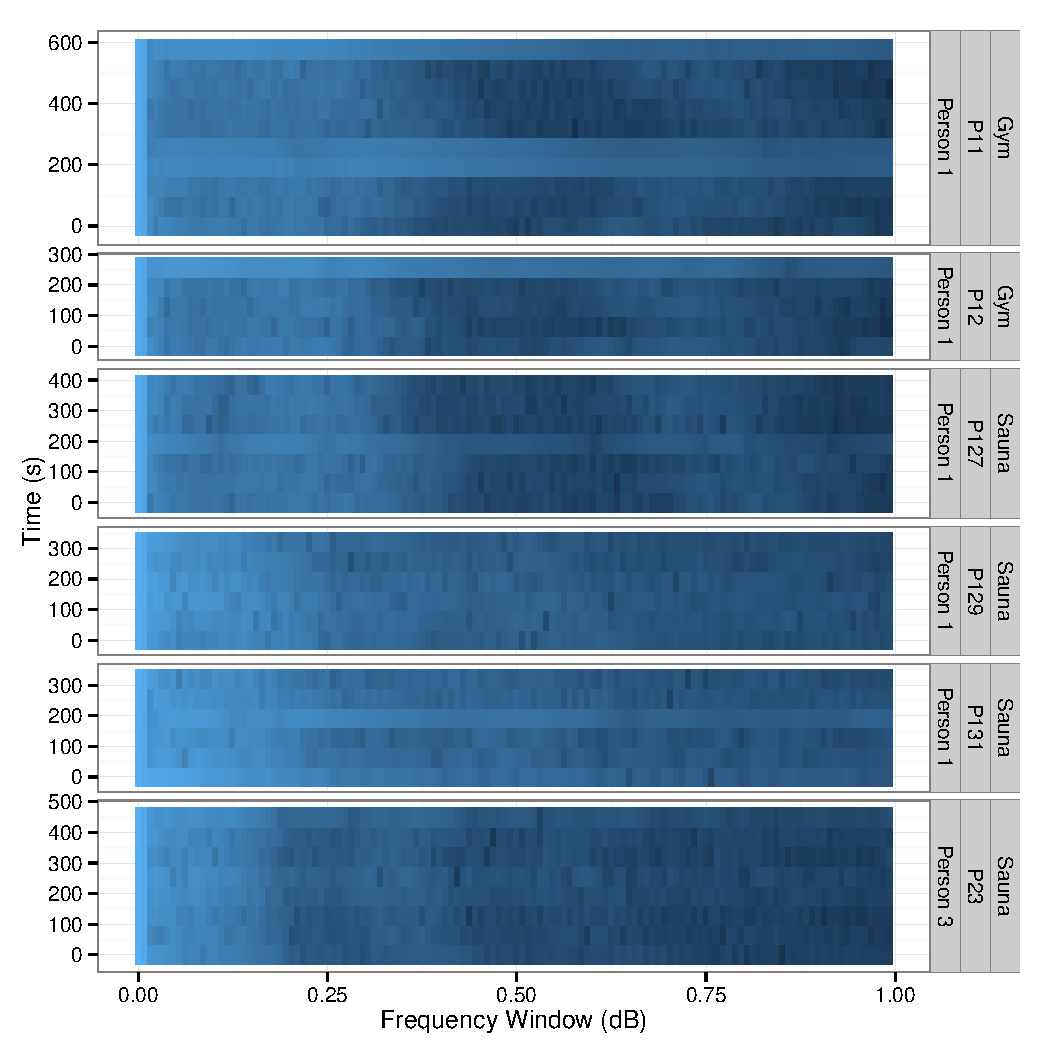
\includegraphics[width=\maxwidth]{figure/dataVizPrint-1} 

\end{knitrout}
\end{columns}
\end{frame}

%% Continue Frame
\begin{frame}[t]{How data looks like}
\begin{columns}[t]
\column{0.6\textwidth}
\begin{knitrout}
\definecolor{shadecolor}{rgb}{0.969, 0.969, 0.969}\color{fgcolor}
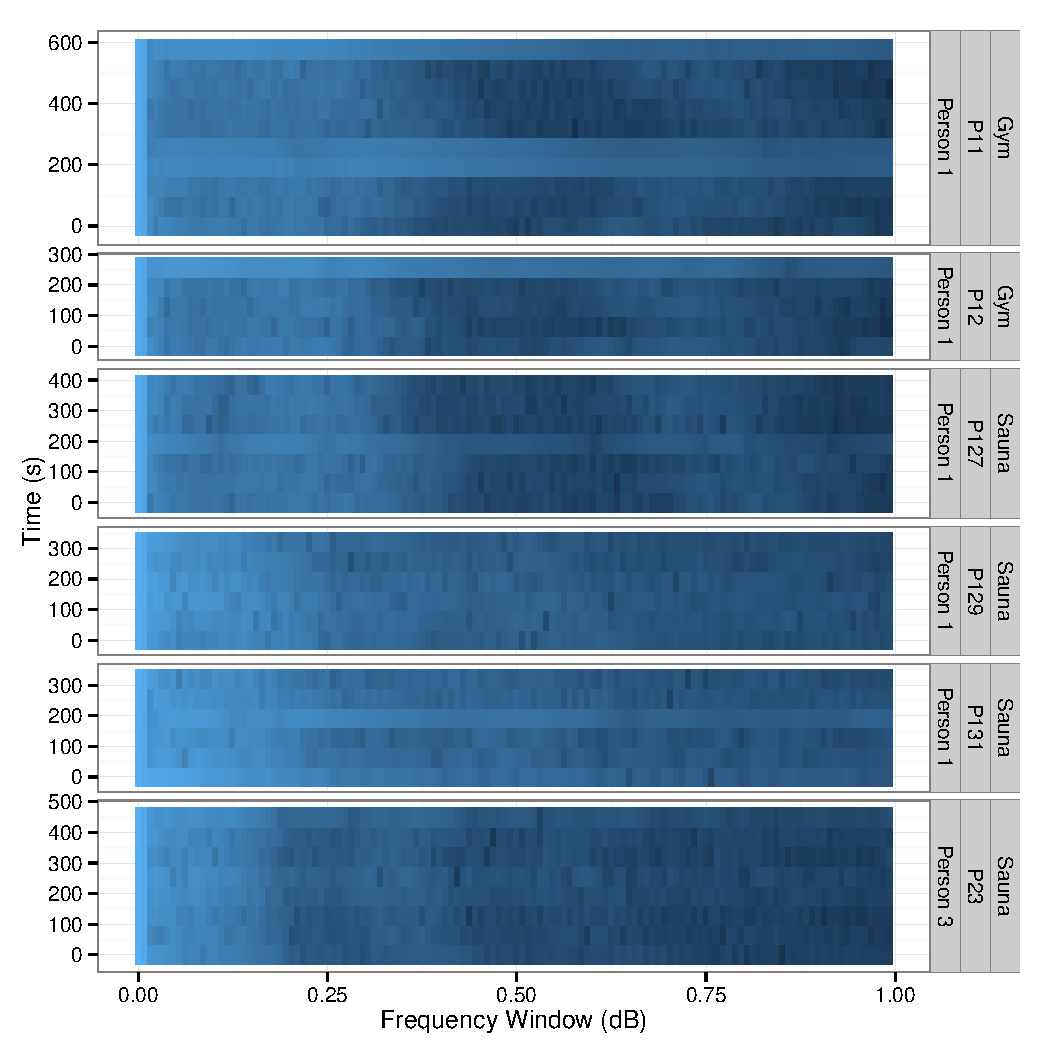
\includegraphics[width=\maxwidth]{figure/dataVizPrint-1} 

\end{knitrout}
\column{0.4\textwidth}
\begin{itemize}[<only@+>]
\item Each block represent a series divided into several windows (rows), 128 columns each with 16 overlaps. The cell contains the frequency values obtained from fast fourier transform
\item Each person may have involved into multiple activities which may have replications
\item Set 1: Each windows are stacked in a row to form a big matrix (may suffer from repeated measurement). This contains different parts of same series in various rows.
\item Set 2: Each series are averaged over different time points. Each row corresponds to one series.
\item Set 3: A person can have multiple series of same activity (replication), the third set is averaged over each person-event conbination. In this case each row corresponds to some specific event for some specific person
\end{itemize}
\end{columns}
\end{frame}

%-=-=-=-=-=-=-=-=-=-=-=-=-=-=-=-=-=-=-=-=-=-=-=-=
%	FRAME: Cross Validation
%-=-=-=-=-=-=-=-=-=-=-=-=-=-=-=-=-=-=-=-=-=-=-=-=
\begin{frame}[c, fragile]{Cross-Validation}
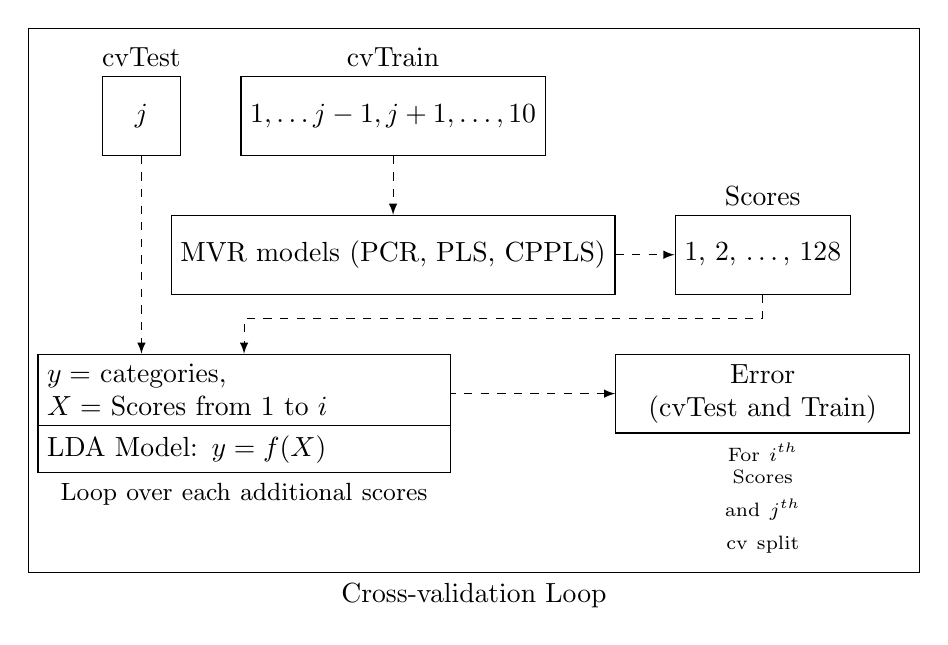
\begin{tikzpicture}[
rectNode/.append style = {draw, rectangle, minimum height = 1cm, minimum width = 1cm},
myArrow/.append style = {->, >=latex, dashed},
node distance = 0.75cm,
]
\visible<1->{
\node[rectNode, label = {[name = cvTestLabel]cvTest}] (cvtest) {$j$};
\node[rectNode, right = of cvtest, label = cvTrain] (cvtrain) {$1,\ldots j-1, j+1, \ldots, 10$};
}
\visible<2->{
\node[rectNode, below = of cvtrain](models) {MVR models (PCR, PLS, CPPLS)};
}
\visible<3->{
\node[rectNode, right = of models, label = Scores](scores) {1, 2, \ldots, 128};
}
\visible<4->{
\node[rectNode, below = of models.195, text width = 5cm, rectangle split, rectangle split parts=2, label = {[text width = 5cm, align = center, name = ldaDataLabel]below:{\small Loop over each additional scores}}](ldaData) {
$y =$ categories, \\$X = $ Scores from $1$ to $i$
	\nodepart{second}
	LDA Model: $y = f(X)$
	};
}
\visible<5->{
\node[text width = 3.5cm, align = center, rectNode, below = of scores, label = {[text width = 1cm, align = center, name = errorLabel]below:{\scriptsize For $i^{th}$ Scores \\ \scriptsize and $j^{th}$ cv split}}](error){Error\\(cvTest and Train)};

\node[fit=(cvTestLabel)(errorLabel)(error)(ldaData)(ldaDataLabel)(scores), draw, label = below:{Cross-validation Loop}] {};
}
%% Arrows

\visible<4->{\draw[myArrow] (cvtest.south) -- (cvtest |- ldaData.north);}
\visible<2->{\draw[myArrow] (cvtrain) -- (models);}
\visible<3->{\draw[myArrow] (models) -- (scores);}
\visible<4->{\draw[myArrow] (scores.south) -- ++(0pt, -3mm)  -| (ldaData.north);}
\visible<5->{\draw[myArrow] (ldaData.east) |- (error);}
\end{tikzpicture}
\end{frame}

\section{Classification with series stack}
% Dealing with First set

% !Rnw root = Presentation.Rnw




%-=-=-=-=-=-=-=-=-=-=-=-=-=-=-=-=-=-=-=-=-=-=-=-=
%	FRAME: Model Error (Test vs Train)
%-=-=-=-=-=-=-=-=-=-=-=-=-=-=-=-=-=-=-=-=-=-=-=-=

\begin{frame}[t]{Training and Cross-validation Errors}
\begin{knitrout}
\definecolor{shadecolor}{rgb}{0.969, 0.969, 0.969}\color{fgcolor}
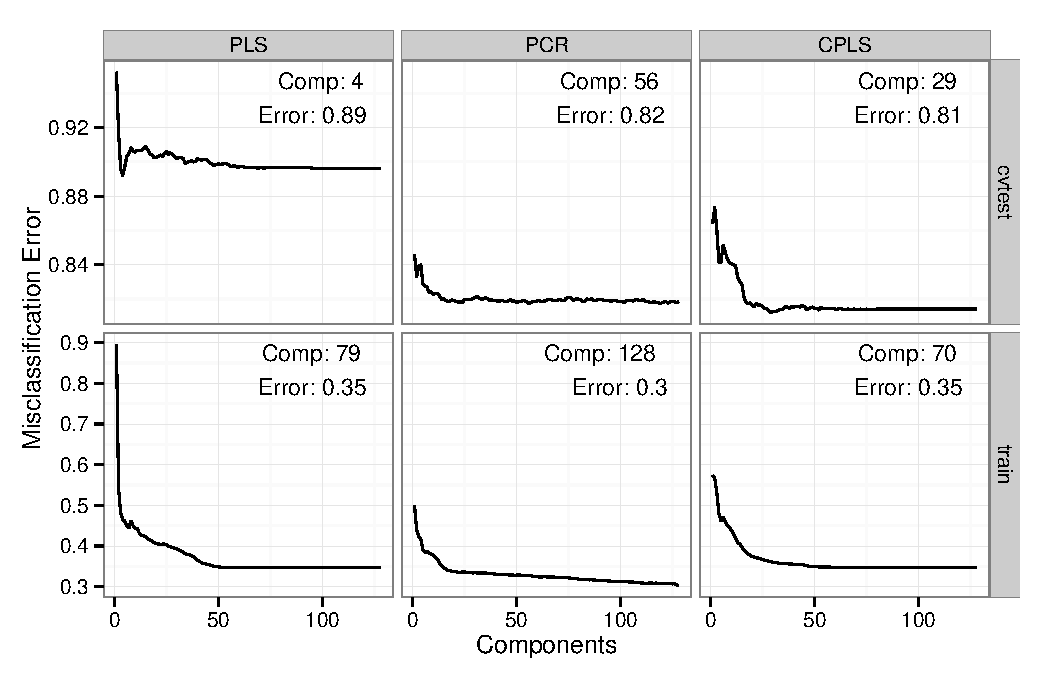
\includegraphics[width=\maxwidth]{figure/Set1ErrorPlot__errPlot-1} 

\end{knitrout}
\end{frame}



%-=-=-=-=-=-=-=-=-=-=-=-=-=-=-=-=-=-=-=-=-=-=-=-=
%	FRAME: Model Misclassification
%-=-=-=-=-=-=-=-=-=-=-=-=-=-=-=-=-=-=-=-=-=-=-=-=

\begin{frame}[c]{Misclassifications}
\only<1>{
{\large Training Misclassifications}
\begin{knitrout}
\definecolor{shadecolor}{rgb}{0.969, 0.969, 0.969}\color{fgcolor}
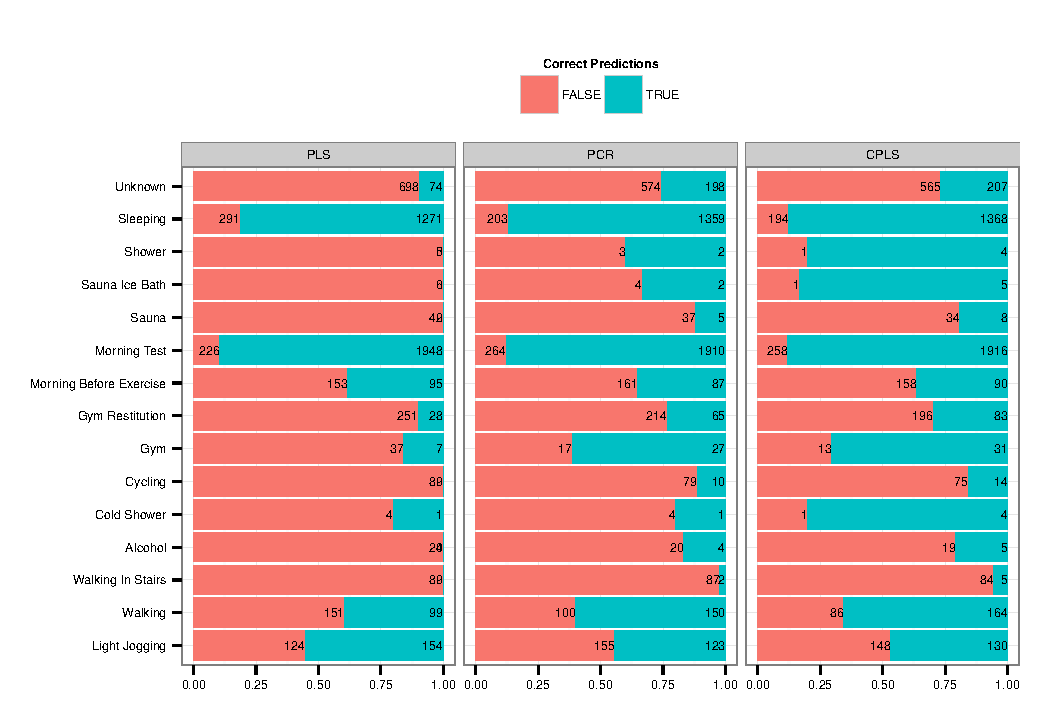
\includegraphics[width=\maxwidth]{figure/Set1MscPlot_1-1} 

\end{knitrout}
}
\only<2>{
{\large Test Misclassification}
\begin{knitrout}
\definecolor{shadecolor}{rgb}{0.969, 0.969, 0.969}\color{fgcolor}
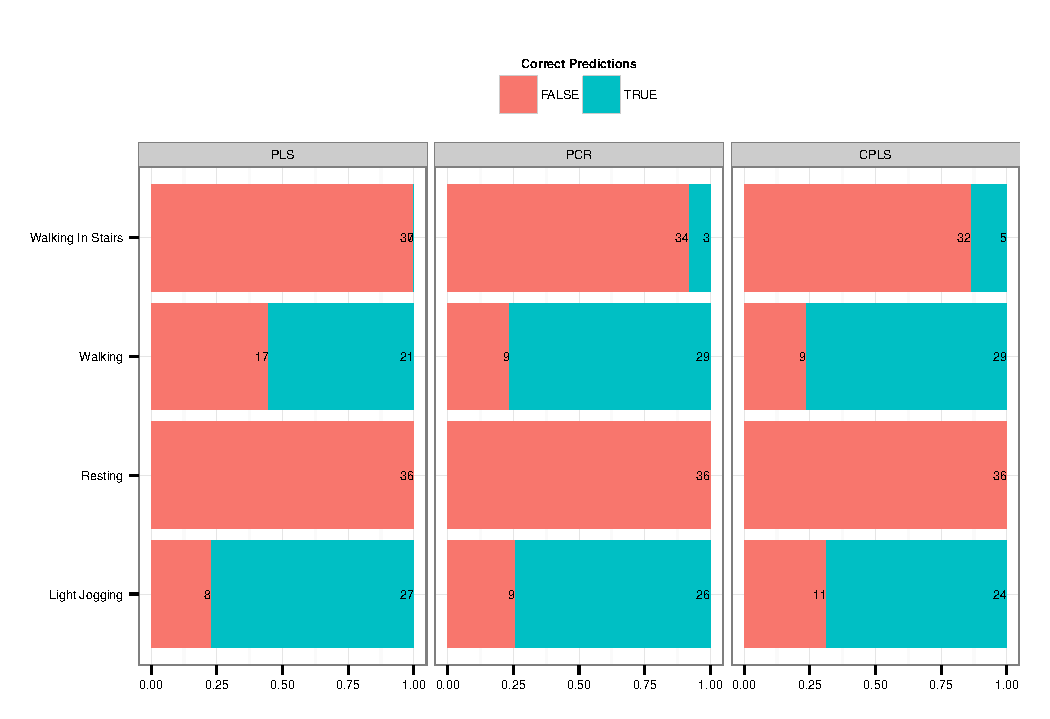
\includegraphics[width=\maxwidth]{figure/Set1MscPlot_2-1} 

\end{knitrout}
}
\end{frame}


%-=-=-=-=-=-=-=-=-=-=-=-=-=-=-=-=-=-=-=-=-=-=-=-=
%	FRAME: Scores for Set1
%-=-=-=-=-=-=-=-=-=-=-=-=-=-=-=-=-=-=-=-=-=-=-=-=

\begin{frame}[c]{Plotting Scores}
\only<1>{
{\large Scoreplot for PCR model}
\begin{knitrout}
\definecolor{shadecolor}{rgb}{0.969, 0.969, 0.969}\color{fgcolor}
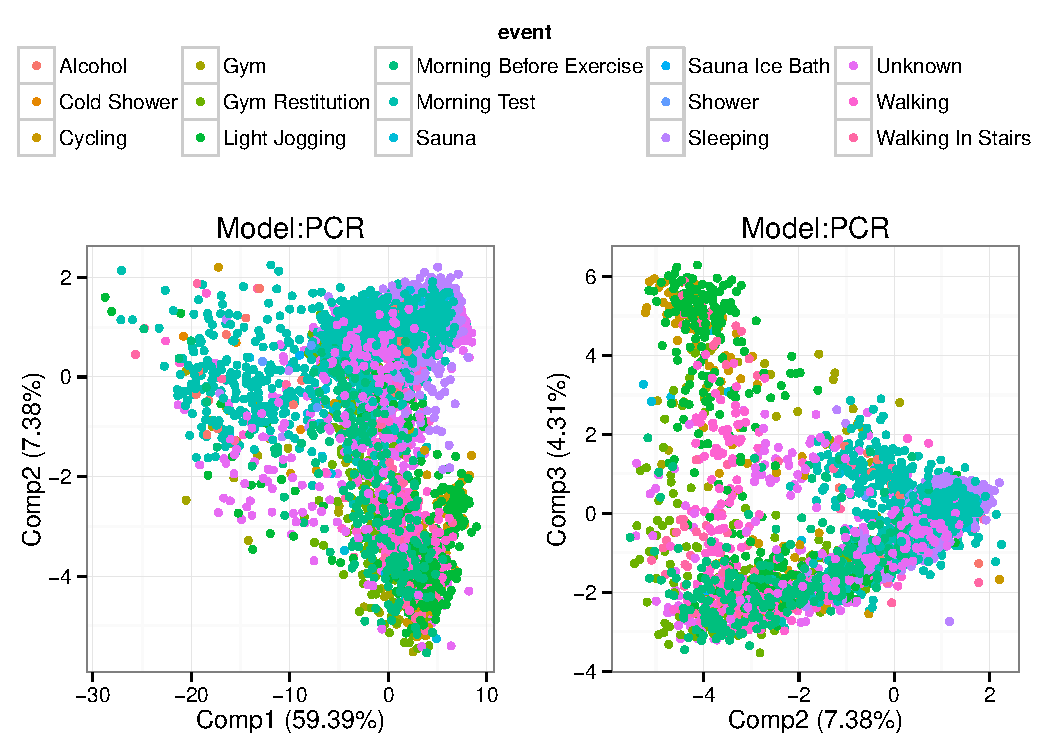
\includegraphics[width=\maxwidth]{figure/Set1ScorePlot1-1} 

\end{knitrout}
}
\only<2>{
{\large Scoreplot for PLS model}
\begin{knitrout}
\definecolor{shadecolor}{rgb}{0.969, 0.969, 0.969}\color{fgcolor}
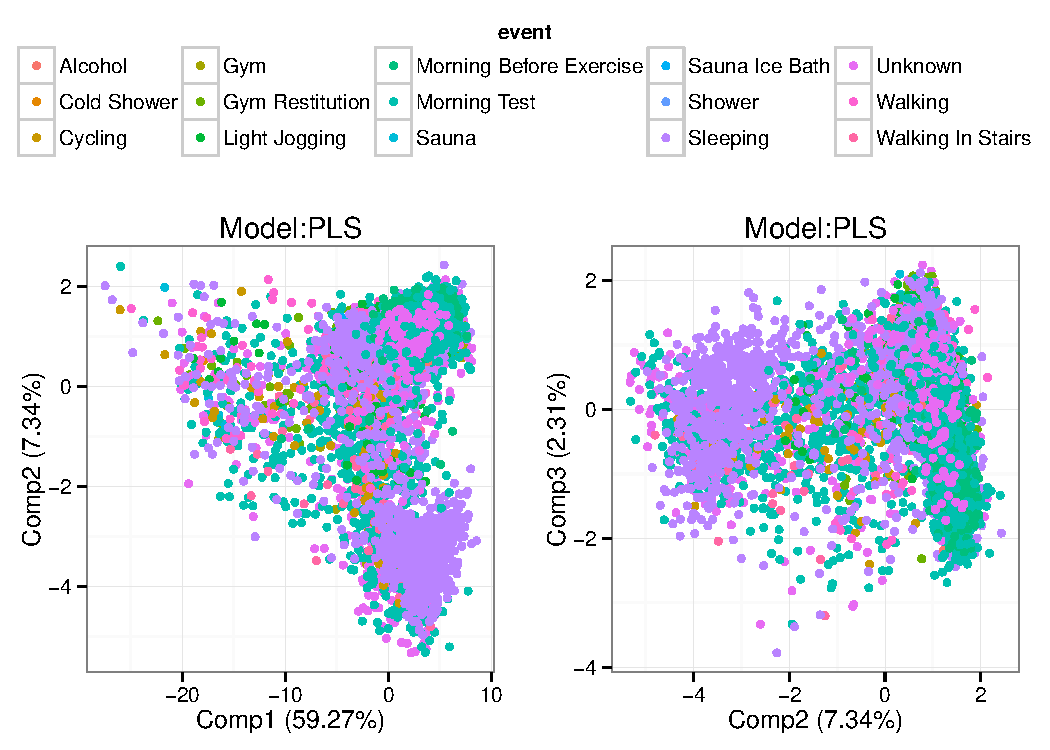
\includegraphics[width=\maxwidth]{figure/Set1ScorePlot2-1} 

\end{knitrout}
}
\only<3>{
{\large Scoreplot for CPPLS model}
\begin{knitrout}
\definecolor{shadecolor}{rgb}{0.969, 0.969, 0.969}\color{fgcolor}
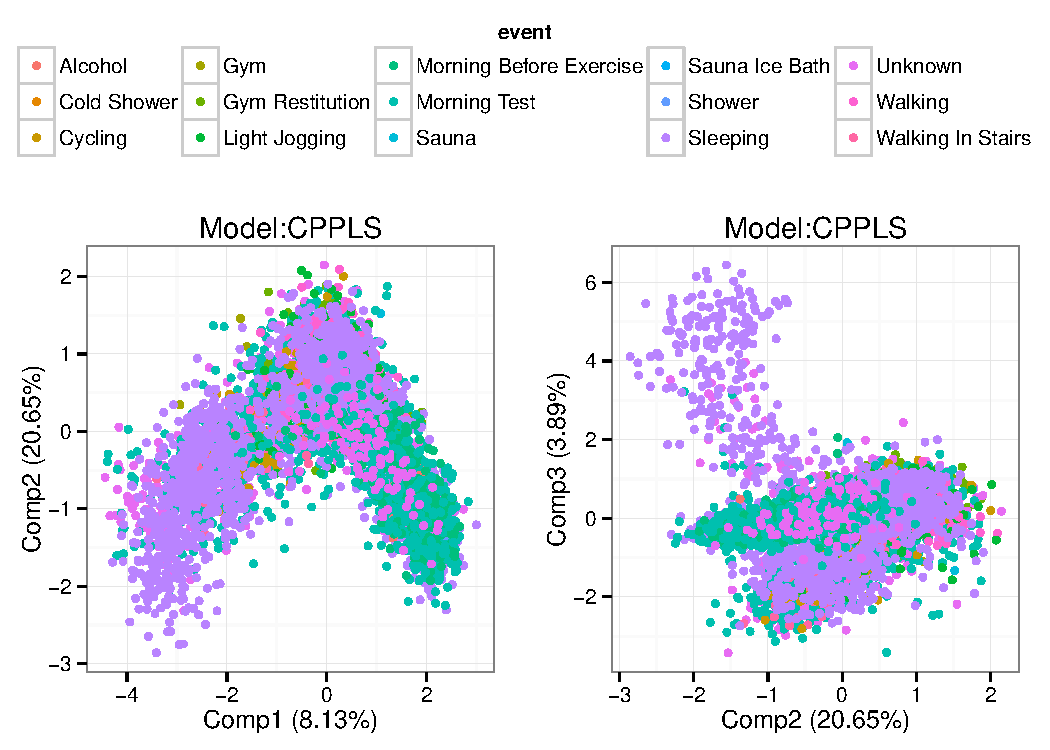
\includegraphics[width=\maxwidth]{figure/Set1ScorePlot3-1} 

\end{knitrout}
}
\end{frame}
\section{Classification with series averaged over Series repetition}

% !Rnw root = Presentation.Rnw




%-=-=-=-=-=-=-=-=-=-=-=-=-=-=-=-=-=-=-=-=-=-=-=-=
%	FRAME: Model Error (Test vs Train)
%-=-=-=-=-=-=-=-=-=-=-=-=-=-=-=-=-=-=-=-=-=-=-=-=

\begin{frame}[t]{Training and Cross-validation Errors}
\begin{knitrout}
\definecolor{shadecolor}{rgb}{0.969, 0.969, 0.969}\color{fgcolor}
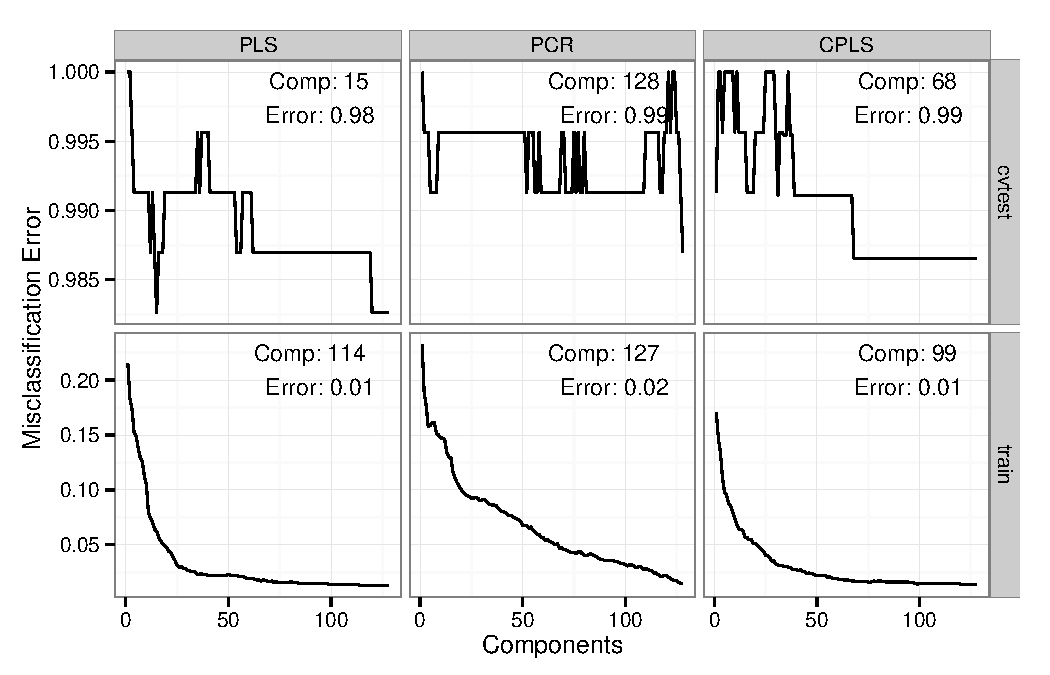
\includegraphics[width=\maxwidth]{figure/Set2ErrorPlot__errPlot-1} 

\end{knitrout}
\end{frame}



%-=-=-=-=-=-=-=-=-=-=-=-=-=-=-=-=-=-=-=-=-=-=-=-=
%	FRAME: Model Misclassification
%-=-=-=-=-=-=-=-=-=-=-=-=-=-=-=-=-=-=-=-=-=-=-=-=

\begin{frame}[c]{Misclassifications}
\only<1>{
{\large Training Misclassifications}
\begin{knitrout}
\definecolor{shadecolor}{rgb}{0.969, 0.969, 0.969}\color{fgcolor}
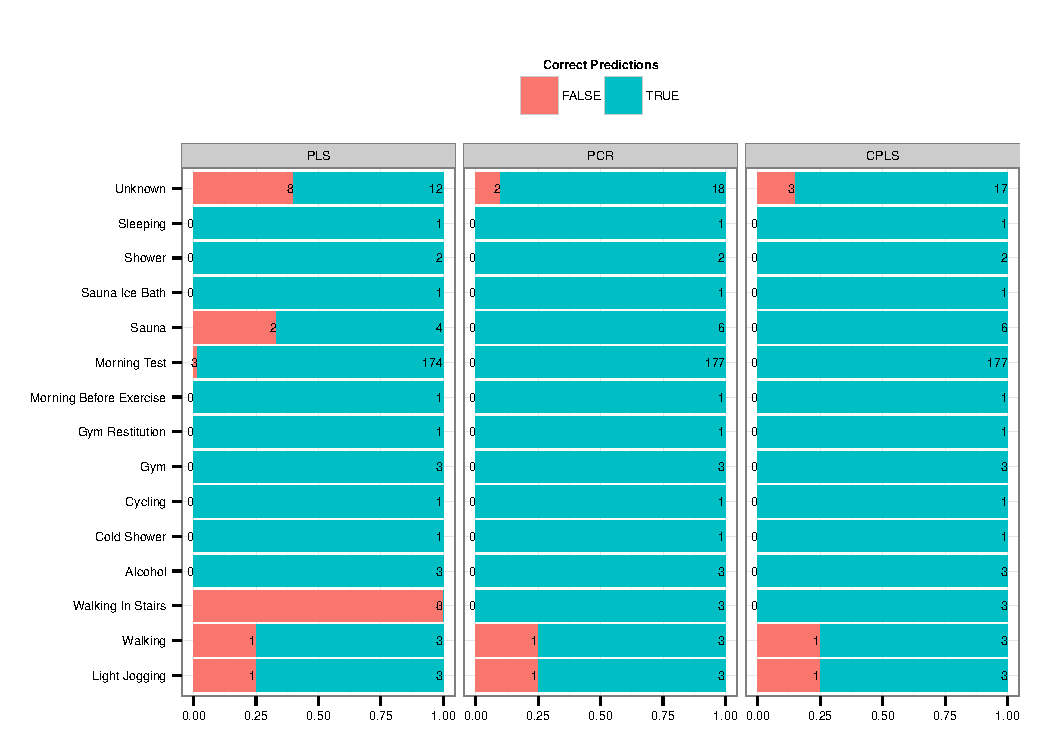
\includegraphics[width=\maxwidth]{figure/Set2MscPlot_1-1} 

\end{knitrout}
}
\only<2>{
{\large Test Misclassification}
\begin{knitrout}
\definecolor{shadecolor}{rgb}{0.969, 0.969, 0.969}\color{fgcolor}
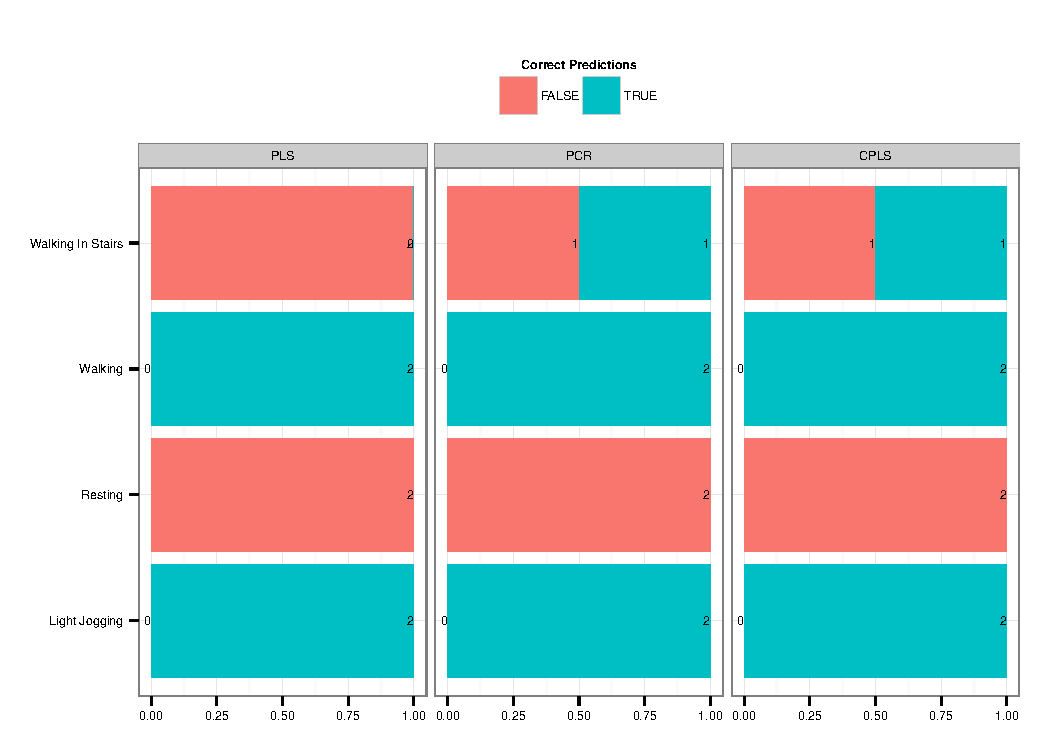
\includegraphics[width=\maxwidth]{figure/Set2MscPlot_2-1} 

\end{knitrout}
}
\end{frame}


%-=-=-=-=-=-=-=-=-=-=-=-=-=-=-=-=-=-=-=-=-=-=-=-=
%	FRAME: Scores for Set2
%-=-=-=-=-=-=-=-=-=-=-=-=-=-=-=-=-=-=-=-=-=-=-=-=

\begin{frame}[c]{Plotting Scores}
\only<1>{
{\large Scoreplot for PCR model}
\begin{knitrout}
\definecolor{shadecolor}{rgb}{0.969, 0.969, 0.969}\color{fgcolor}
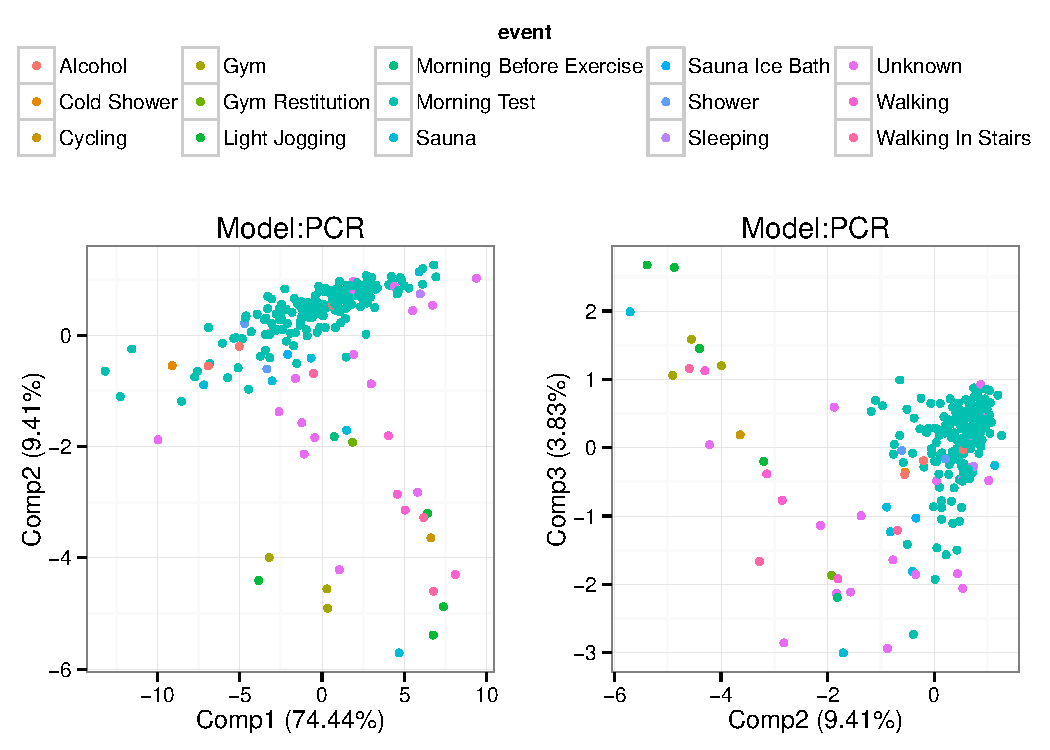
\includegraphics[width=\maxwidth]{figure/Set2ScorePlot1-1} 

\end{knitrout}
}
\only<2>{
{\large Scoreplot for PLS model}
\begin{knitrout}
\definecolor{shadecolor}{rgb}{0.969, 0.969, 0.969}\color{fgcolor}
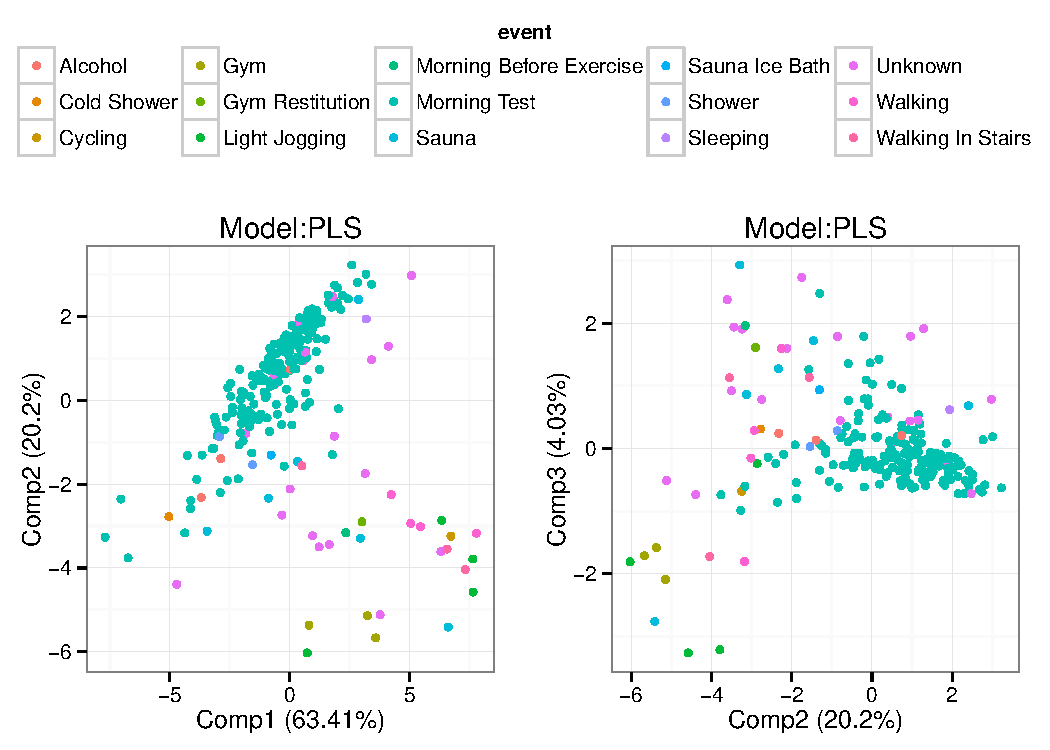
\includegraphics[width=\maxwidth]{figure/Set2ScorePlot2-1} 

\end{knitrout}
}
\only<3>{
{\large Scoreplot for CPPLS model}
\begin{knitrout}
\definecolor{shadecolor}{rgb}{0.969, 0.969, 0.969}\color{fgcolor}
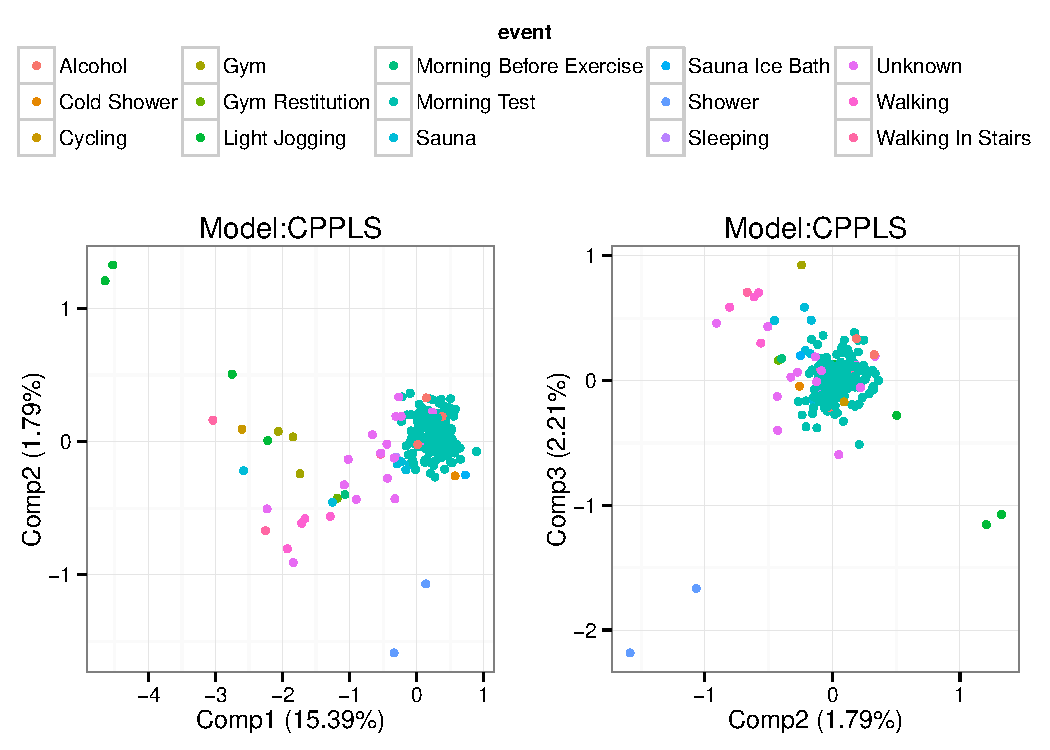
\includegraphics[width=\maxwidth]{figure/Set2ScorePlot3-1} 

\end{knitrout}
}
\end{frame}
\section{Classification with series averaged over Person-Event Combination}

% !Rnw root = Presentation.Rnw





%-=-=-=-=-=-=-=-=-=-=-=-=-=-=-=-=-=-=-=-=-=-=-=-=
%	FRAME: Model Error (Test vs Train)
%-=-=-=-=-=-=-=-=-=-=-=-=-=-=-=-=-=-=-=-=-=-=-=-=

\begin{frame}[t]{Training and Cross-validation Errors}
\begin{knitrout}
\definecolor{shadecolor}{rgb}{0.969, 0.969, 0.969}\color{fgcolor}
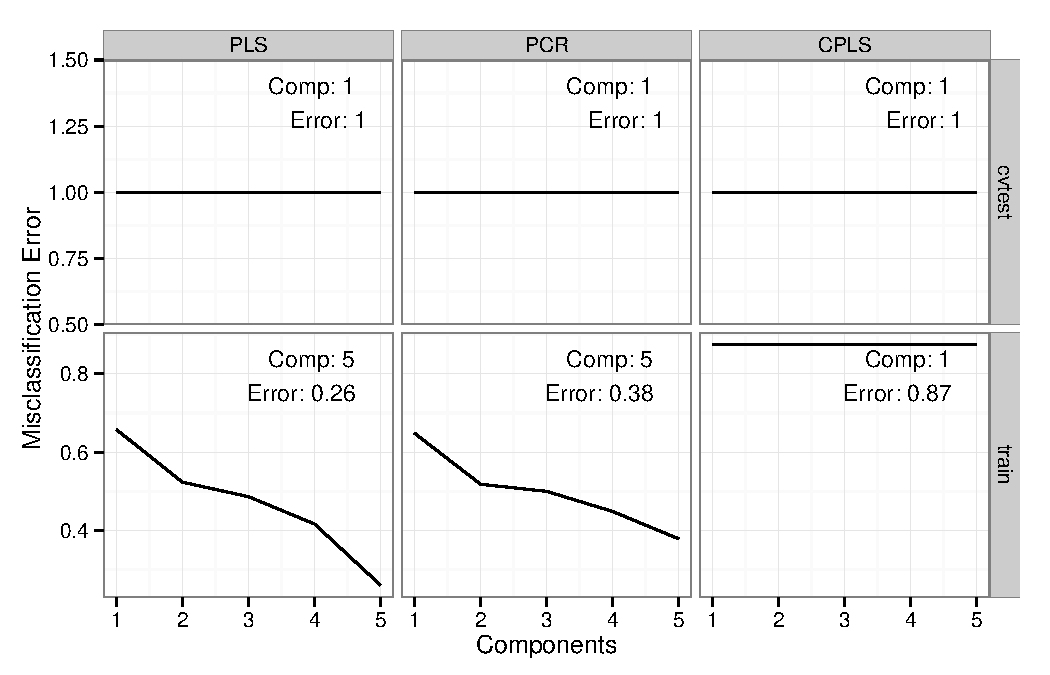
\includegraphics[width=\maxwidth]{figure/Set3ErrorPlot__errPlot-1} 

\end{knitrout}
\end{frame}



%-=-=-=-=-=-=-=-=-=-=-=-=-=-=-=-=-=-=-=-=-=-=-=-=
%	FRAME: Model Misclassification
%-=-=-=-=-=-=-=-=-=-=-=-=-=-=-=-=-=-=-=-=-=-=-=-=

\begin{frame}[c]{Misclassifications}
\only<1>{
{\large Training Misclassifications}
\begin{knitrout}
\definecolor{shadecolor}{rgb}{0.969, 0.969, 0.969}\color{fgcolor}
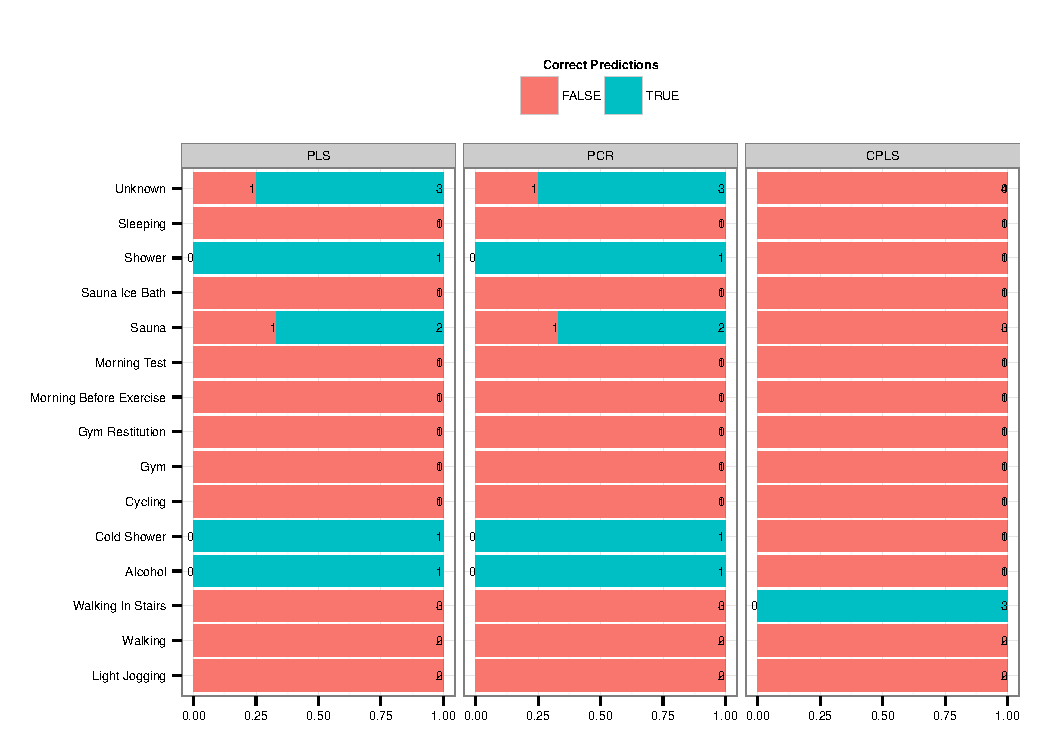
\includegraphics[width=\maxwidth]{figure/Set3MscPlot_1-1} 

\end{knitrout}
}
\only<2>{
{\large Test Misclassification}
\begin{knitrout}
\definecolor{shadecolor}{rgb}{0.969, 0.969, 0.969}\color{fgcolor}
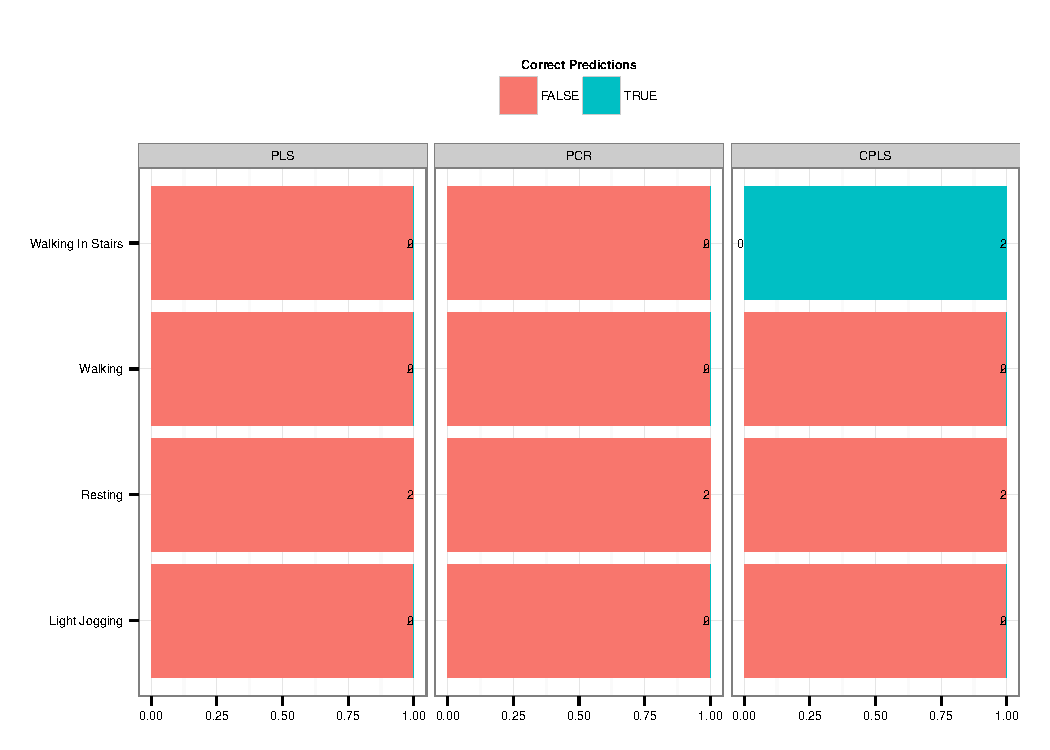
\includegraphics[width=\maxwidth]{figure/Set3MscPlot_2-1} 

\end{knitrout}
}
\end{frame}


%-=-=-=-=-=-=-=-=-=-=-=-=-=-=-=-=-=-=-=-=-=-=-=-=
%	FRAME: Scores for Set3
%-=-=-=-=-=-=-=-=-=-=-=-=-=-=-=-=-=-=-=-=-=-=-=-=

\begin{frame}[c]{Plotting Scores}
\only<1>{
{\large Scoreplot for PCR model}
\begin{knitrout}
\definecolor{shadecolor}{rgb}{0.969, 0.969, 0.969}\color{fgcolor}
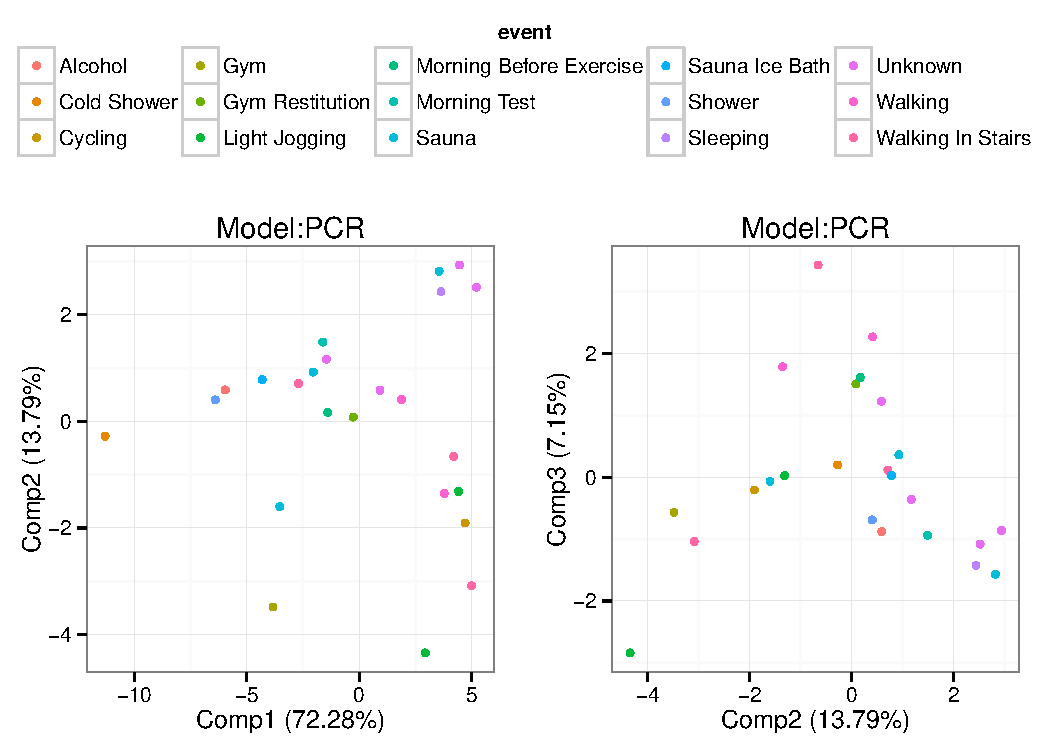
\includegraphics[width=\maxwidth]{figure/Set3ScorePlot1-1} 

\end{knitrout}
}
\only<2>{
{\large Scoreplot for PLS model}
\begin{knitrout}
\definecolor{shadecolor}{rgb}{0.969, 0.969, 0.969}\color{fgcolor}
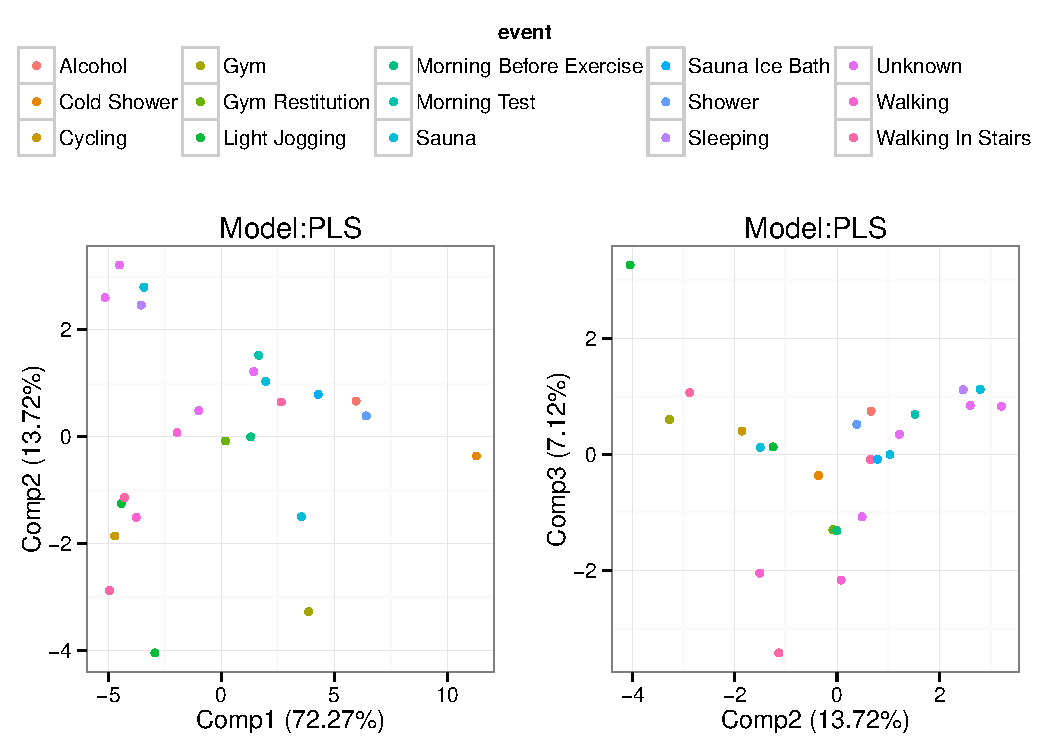
\includegraphics[width=\maxwidth]{figure/Set3ScorePlot2-1} 

\end{knitrout}
}
\only<3>{
{\large Scoreplot for CPPLS model}
\begin{knitrout}
\definecolor{shadecolor}{rgb}{0.969, 0.969, 0.969}\color{fgcolor}
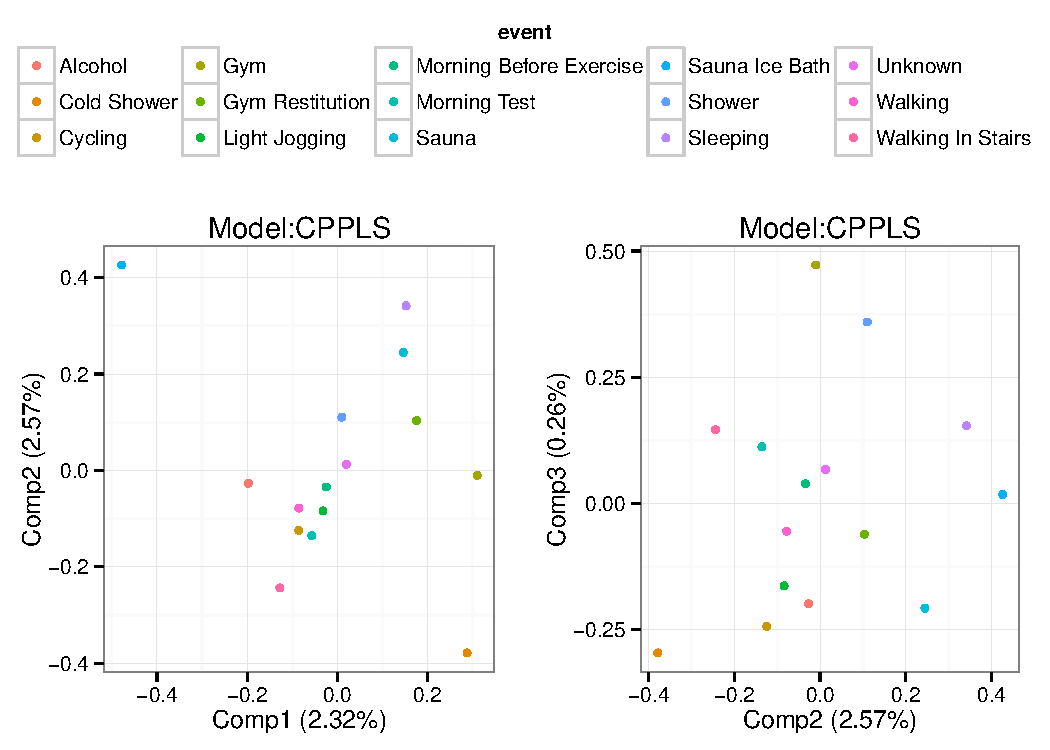
\includegraphics[width=\maxwidth]{figure/Set3ScorePlot3-1} 

\end{knitrout}
}
\end{frame}

%-=-=-=-=-=-=-=-=-=-=-=-=-=-=-=-=-=-=-=-=-=-=-=-=
%	FRAME: Model Comparison with Misclassification Error
%-=-=-=-=-=-=-=-=-=-=-=-=-=-=-=-=-=-=-=-=-=-=-=-=

\section{Some Comparison}
\begin{frame}[t]{Misclassification Errors}

\begin{knitrout}
\definecolor{shadecolor}{rgb}{0.969, 0.969, 0.969}\color{fgcolor}\begin{figure}
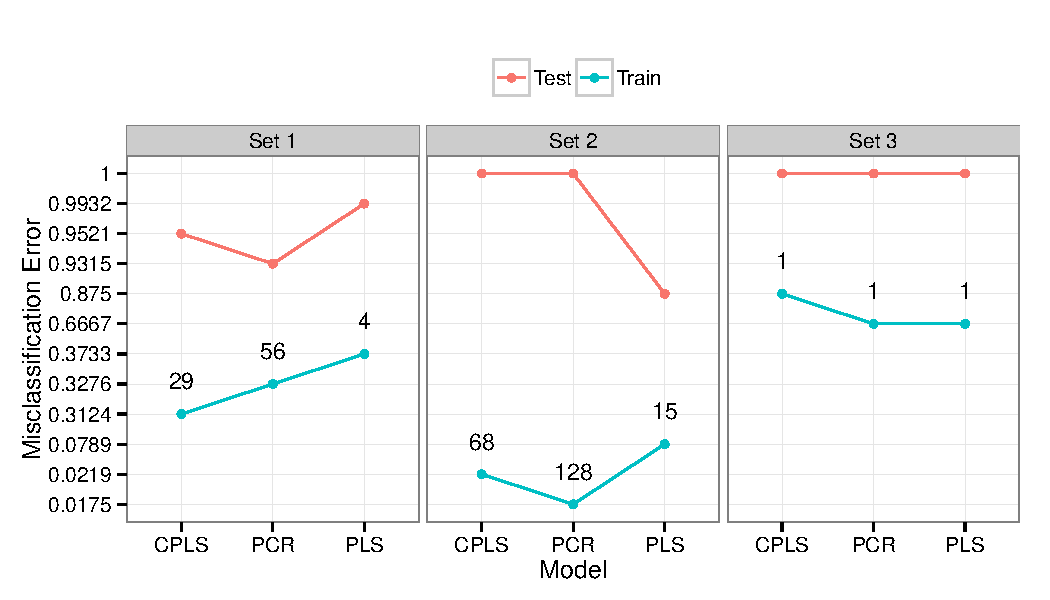
\includegraphics[width=\maxwidth]{figure/mscErrorPlot-1} \caption[Training and Test Misclassification Error for all the three models]{Training and Test Misclassification Error for all the three models. The LDA models were fitted with the scores obtained from three models with components (number above each points) needed to get minimum cross-validation error.}\label{fig:mscErrorPlot}
\end{figure}


\end{knitrout}
\end{frame}

%-=-=-=-=-=-=-=-=-=-=-=-=-=-=-=-=-=-=-=-=-=-=-=-=
%	FRAME: References
%-=-=-=-=-=-=-=-=-=-=-=-=-=-=-=-=-=-=-=-=-=-=-=-=
\begin{frame}[c]{References}
\nocite{indahl2009canonical,R-data.table,wickham2006ggplot,R-knitr,martens2001multivariate,martens1992multivariate,wickham2012reshape2,R-signal}
\printbibliography
\end{frame}

\end{document}
